\noindent
\includegraphics[height=1.25cm]{images/pictograms/benchmark}
\includegraphics[height=1.25cm]{images/pictograms/under_construction}
\includegraphics[height=1.25cm]{images/pictograms/FDM}
\includegraphics[height=1.25cm]{images/pictograms/paraview}
\includegraphics[height=1.25cm]{images/pictograms/streamfunction}

%%%%%%%%%%%%%%%%%%%%%%%%%%%%%%%%%%%%%%%%%%%%%%%%%%%%%%%%%%%%%%%%%%%%%%%%%%%%%%%%%%%%%%%%%%%%%%%%%%%

\begin{flushright} {\tiny {\color{gray} python\_codes/fieldstone\_154/text.tex}} \end{flushright}

%\lstinputlisting[language=bash,basicstyle=\small]{python_codes/fieldstone_154/keywords.key}

\par\noindent\rule{\textwidth}{0.4pt}

\begin{center}
\inpython
{\small Code: \url{https://github.com/cedrict/fieldstone/tree/master/python_codes/fieldstone_154}}
\end{center}

\par\noindent\rule{\textwidth}{0.4pt}

{\bf \color{teal} Purpose}: implement and document bla bla 

\par\noindent\rule{\textwidth}{0.4pt}

%%%%%%%%%%%%%%%%%%%%%%%%%%%%%%%%%%%%%%%%%%%%%%%%%%%%%%%%%%%%%%%%%%%%%%%%%%%%%%%%%%%%%%%%%%%%%%%%%%%


%%%%%%%%%%%%%%%%%%%%%%%%%%
\section*{Poiseuille flow benchmark}

In what follows we consider a 2D domain of dimensions $L_x \times L_y$ in which 
a fluid flows in the absence of gravitational forces (the flow is entirely driven by 
the boundary conditions impose on the left - the 'inlet'). The domain is discretised by means of a regular grid 
of $nnx \times nny$ points. 

The default parameters are $L_x=5$, $L_y=1$, $\delta t=0.002$, $t_{\text{final}}=5$,
$u(y)=y(1-y)$, mesh is $101\times 21$ nodes,$\Renb=400$.


%%%%%%%%%%%%%%%%%%%%%%%%%%%%%%%%
\subsection*{Boundary conditions}


In the context of this experiment, we have four boundaries (left, right, bottom and top). 
\begin{itemize}

\item The left one (the inlet) is characterised by $\vec\upnu=(u_0,0)$ for $y\in[0,L_y]$, so that 
\begin{equation}
\omega(0,y) = \partial_x v-\partial_y u = 0
\label{eq:omega1}
\end{equation}
Likewise $u=\frac{\partial \Psi}{\partial y}=u_0$ so $\Psi$ is a linear function of $y$ on this boundary and since $v=-\frac{\partial \Psi}{\partial x}=0$ then $\Psi$ does not depend on $x$. 

\item The right one is such that a laminar flow exits there. In this case $\vec\upnu=(u(y),0)$ so that
$\omega_{\text right} = \partial_x v-\partial_y u = -\partial_y u $. This is not particularly helpful since we do not know the exact form of $u(y)$, but we also have 
\begin{equation}
\frac{\partial \omega }{\partial x}(L_x,y) =
\frac{\partial^2 v}{\partial x^2}
-\frac{\partial^2 u}{\partial x\partial y}
= -\frac{\partial^2 u}{\partial x\partial y} =0
\label{eq:omega2}
\end{equation}
since $u$ is only a function of $y$.

\item At the bottom, we have $u=v=0$ (no-slip boundary conditions) for $x>0$ (the lower left corner 'belongs' to the left boundary).
As such it is not straightforward to establish the value of the vorticity there. 
However, let us look at a Taylor expansion of $\Psi(x,y)$ at a point with coordinates $(x,h)$ just above 
the bottom boundary:
\[
\Psi(x,h) = \Psi(x,0) + h \frac{\partial \Psi}{\partial y}(x,0)  
+ \frac{h^2}{2}  \frac{\partial^2 \Psi}{\partial y^2} (x,0) + ...
\]
Since by definition $u=\frac{\partial \Psi}{\partial y}$ and $u=0$ on this boundary we are left with:
\[
\Psi(x,h) = \Psi(x,0) + \frac{h^2}{2}  \frac{\partial^2 \Psi}{\partial y^2}(x,0) + ...
\]
Also, we have the following relationship:
$
\vec\nabla^2 \Psi=
\frac{\partial^2 \Psi}{\partial x^2 }
+\frac{\partial^2 \Psi}{\partial y^2 } = -\omega
$ and since at the wall $\Psi$ is independent of $x$ ($0=v=-\partial_x \Psi$) the second-order $x$-derivative is zero, so that $\frac{\partial^2 \Psi}{\partial y^2 } = -\omega$ and then
\[
\Psi(x,h) = \Psi(x,0) - \frac{h^2}{2}  \omega(x,0) + ...
\]
In discrete form\footnote{I here adopt python conventions, $j=0$ is the row of nodes at the 
bottom of the domain, while $nny-1$ is the row of nodes at the top.}:
\[
\Psi_{i,j+1} = \Psi_{i,j} - \frac{h^2}{2} \omega_{i,j} \qquad \text{for} \quad  j=0
\]
and then
\begin{equation}
\omega_{i,0} = \frac{2}{h^2} (\Psi_{i,0} -\Psi_{i,1} )  
\label{eq:omega3}
\end{equation}
Also $u=\frac{\partial \Psi}{\partial y}=0$ and $v=-\frac{\partial \Psi}{\partial x}=0$ on this boundary so $\Psi$ is constant (but not necessarily zero). 



\item We can use the same approach at the top boundary (also no-slip boundary conditions, with the upper left corner belonging to the left boundary) by taking a Taylor expansion at a point with coordinates $(x,L_y-h)$:
\[
\Psi(x,L_y-h) = \Psi(x,L_y) - h \frac{\partial \Psi}{\partial y}(x,L_y)  
+ \frac{h^2}{2}  \frac{\partial^2 \Psi}{\partial y^2} (x,L_y) + ...
\]
which becomes (since $u=\partial_y \Psi=0$)
\[
\Psi(x,L_y-h) = \Psi(x,L_y) 
-\omega (x,L_y) + ...
\]
and then
\begin{equation}
\omega_{i,nny-1} = \frac{2}{h^2} (\Psi_{i,nny-1} -\Psi_{i,nny-2} )  
\label{eq:omega4}
\end{equation}
Also $u=\frac{\partial \Psi}{\partial y}=0$ and $v=-\frac{\partial \Psi}{\partial x}=0$ on this boundary so $\Psi$ is constant (but not necessarily zero). 

\end{itemize}

%%%%%%%%%%%%%%%%%%%%%%%%%%%%%%%%
\subsection*{The algorithm}




Because of the presence of no-slip boundary conditions, the algorithm goes as follows. 
At the beginning zero all fields, i.e. $u=v=\omega=\Psi=0$.

\begin{center}
\begin{verbatim}
LTTTTTTTTTTTTTTTTTTTTTTTTR
L                        R
L                        R 
L                        R 
LBBBBBBBBBBBBBBBBBBBBBBBBR
\end{verbatim}
\end{center}

\begin{enumerate}

\item solve $\Delta \Psi = -\omega$ 
\[
\frac{\Psi_{\color{brown} i-1,j}-2\Psi_{\color{brown} i,j}+\Psi_{\color{brown} i+1,j}}{h_x^2}
+
\frac{\Psi_{\color{brown} i,j-1}-2\Psi_{\color{brown} i,j}+\Psi_{\color{brown} i,j+1}}{h_y^2}
=
-\omega_{\color{brown} i,j}
\]
or,
\[
\frac{1}{h_x^2} \Psi_{\color{brown} i-1,j}
+\frac{1}{h_y^2} \Psi_{\color{brown} i,j-1}
-\left(\frac{2}{h_x^2}+\frac{2}{h_y^2} \right)\Psi_{\color{brown} i,j}
+\frac{1}{h_x^2} \Psi_{\color{brown} i+1,j}
+\frac{1}{h_y^2} \Psi_{\color{brown} i,j+1}
=
-\omega_{\color{brown}  i,j}
\]
so that we obtain a pentadiagonal matrix.

About the boundary conditions:
Since $\Psi$ is known up to a constant (and is constant) at the bottom, we arbitrarily fix $\Psi=0$. Since $\Psi$ is linear and only depends on $y$ on the inlet (left boundary) then $\Psi(y)=u_0 y$ there. This means that at the top $\Psi$ is constant and equal to $u_0 L_y$. At the outlet we have $\partial \Psi/\partial x=0$. This last condition is 
compatible with the values on the top and bottom so no need to think about the corners.

\item compute velocity field at interior nodes with centered stencils
\[
u^n_{\color{brown} i,j} = \frac{\partial \Psi^n_{\color{brown} i,j}}{\partial y} = \frac{\Psi^n_{\color{brown} i,j+1}-\Psi^n_{\color{brown} i,j-1}}{2h_y}
\qquad\qquad
v^n_{\color{brown} i,j} = -\frac{\partial \Psi^n_{\color{brown} i,j}}{\partial x} = -\frac{\Psi^n_{\color{brown} i+1,j}-\Psi^n_{\color{brown} i-1,j}}{2 h_x}
\]
Velocity is analytically known on the bottom, left and top boundaries. 
On the right boundary we have $v=0$ (that stems from us imposing $\partial \Psi/\partial x=0$ there) and we can compute $u_{i,j}$ there using the formula above for 
$j\in[1,nny-2]$. 


\item Having obtained $\vec\upnu^n$ we can solve the vorticity equation stemming for the time-dependent Navier-Stokes equation (see Section~\ref{MMM-ss:streamfunctionNS}):
\[
\frac{\partial \omega}{\partial t} + \vec\upnu \cdot \vec\nabla \omega= 
\frac{1}{\Renb} \left(\frac{\partial^2 \omega}{\partial x^2}+\frac{\partial^2 \omega}{\partial y^2} \right)
\]
We discretise the time derivative as follows:
\[
\frac{\partial \omega}{\partial t} = \frac{\omega^n-\omega^{n-1}}{\delta t}
\]
and then write
\[
\frac{\omega_{{\color{brown} i,j}}^n-\omega_{{\color{brown} i,j}}^{n-1}}{\delta t}
+ u_{\color{brown} i,j} \frac{\omega^n_{\color{brown} i+1,j}-\omega^n_{\color{brown} i-1,j}}{2h_x}
+ v_{\color{brown} i,j} \frac{\omega^n_{\color{brown} i,j+1}-\omega^n_{\color{brown} i,j-1}}{2h_y}
-\frac{1}{\Renb} 
\left(
\frac{\omega^n_{\color{brown} i-1,j}-2\omega^n_{\color{brown} i,j}+\omega^n_{\color{brown} i+1,j}}{h_x^2}
+
\frac{\omega^n_{\color{brown} i,j-1}-2\omega^n_{\color{brown} i,j}+\omega^n_{\color{brown} i,j+1}}{h_y^2}
\right)=0
\]
or,
\[
\omega^n_{\color{brown} i,j}
+ \frac{u_{\color{brown} i,j} 
\delta t}{2 h_x} (\omega^n_{\color{brown} i+1,j}-\omega^n_{\color{brown} i-1,j})
+ \frac{v_{\color{brown} i,j} 
\delta t}{2 h_y} (\omega^n_{\color{brown} i,j+1}-\omega^n_{\color{brown} i,j-1})
-\frac{\delta t}{\Renb} 
\left(
\frac{\omega^n_{\color{brown} i-1,j}
-2\omega^n_{\color{brown} i,j}
+\omega^n_{\color{brown} i+1,j}}{h_x^2}
+
\frac{\omega^n_{\color{brown} i,j-1}
-2\omega^n_{\color{brown} i,j}
+\omega^n_{\color{brown} i,j+1}}{h_y^2}
\right)
=\omega^{n-1}_{\color{brown} i,j}
\]
that is,
\begin{eqnarray}
\left(-\frac{u_{\color{brown} i,j} \delta t}{2 h_x} -\frac{\delta t}{h_x^2 \Renb} \right) \omega_{{\color{brown} i-1,j}}^n
+\left(-\frac{v_{\color{brown} i,j} \delta t}{2 h_y} -\frac{\delta t}{h_y^2 \Renb} \right) \omega_{{\color{brown} i,j-1}}^n&& \nn\\
+\left( \frac{u_{\color{brown} i,j} \delta t}{2 h_x} -\frac{\delta t}{h_x^2 \Renb}\right) \omega_{{\color{brown} i+1,j}}^n
+\left( \frac{v_{\color{brown} i,j} \delta t}{2 h_y} -\frac{\delta t}{h_y^2 \Renb}\right) \omega_{{\color{brown} i,j+1}}^n && \nn\\
+\left( 1 +\frac{2 \delta t}{h_x^2 \Renb} +\frac{2 \delta t}{h_y^2 \Renb}   \right)\omega_{{\color{brown} i,j}}^n
&=&\omega_{{\color{brown} i,j}}^{n-1} 
\end{eqnarray}
Again, a pentadiagonal matrix.

Note that if we only consider the steady-state equations, then $\partial \omega/\partial t \rightarrow 0$ so that we obtain:
\begin{eqnarray}
\left(-\frac{u_{\color{brown} i,j} }{2 h_x} -\frac{1}{h_x^2 \Renb} \right) \omega_{{\color{brown} i-1,j}}^n
+\left(-\frac{v_{\color{brown} i,j} }{2 h_y} -\frac{1}{h_y^2 \Renb} \right) \omega_{{\color{brown} i,j-1}}^n && \nn\\
+\left(\frac{u_{\color{brown} i,j} }{2 h_x} -\frac{1}{h_x^2 \Renb}\right) \omega_{{\color{brown} i+1,j}}^n
+\left(\frac{v_{\color{brown} i,j} }{2 h_y} -\frac{1}{h_y^2 \Renb}\right) \omega_{{\color{brown} i,j+1}}^n && \nn\\
+\left(\frac{2 }{h_x^2 \Renb} +\frac{2 }{h_y^2 \Renb}   \right)\omega_{{\color{brown} i,j}}^n
&=&0
\end{eqnarray}
Finally, if we only wish to solve the Stokes equations, then the advection (inertia) term also disappears and we are left with 
\[
\frac{\partial^2 \omega}{\partial x^2}+\frac{\partial^2 \omega}{\partial y^2} 
=0
\]
and we see that the Reynolds number $\Renb$ is no more a parameter of the PDE. 
It translates into
\begin{eqnarray}
\left(- \frac{1}{h_x^2 } \right) \omega_{{\color{brown} i-1,j}}^n
+\left(- \frac{1}{h_y^2 } \right) \omega_{{\color{brown} i,j-1}}^n 
+\left(-\frac{1}{h_x^2 }\right) \omega_{{\color{brown} i+1,j}}^n
+\left(- \frac{1}{h_y^2 }\right) \omega_{{\color{brown} i,j+1}}^n 
+\left(\frac{2 }{h_x^2} +\frac{2 }{h_y^2}   \right)\omega_{{\color{brown} i,j}}^n
&=&0
\end{eqnarray}

Concerning the boundary conditions we use 
Eqs.~\eqref{eq:omega1},\eqref{eq:omega2},\eqref{eq:omega3},\eqref{eq:omega4} above, i.e.
\begin{eqnarray}
\omega_{0,j} &=& 0  \qquad \text{left}\\
\frac{\partial \omega_{nnx-1,j}}{\partial x} &=& 0  \qquad \text{right}\\
\omega_{i,0} &=&  \frac{2}{h^2} (\Psi_{i,0} -\Psi_{i,1} ) \qquad \text{bottom}\\
\omega_{i,nny-1} &=& \frac{2}{h^2} (\Psi_{i,nny-1} -\Psi_{i,nny-2} ) \qquad \text{top}
\end{eqnarray}


\item if $u$, $v$, $\omega$ and $\Psi$ not converged go to 1

\end{enumerate}



\begin{center}
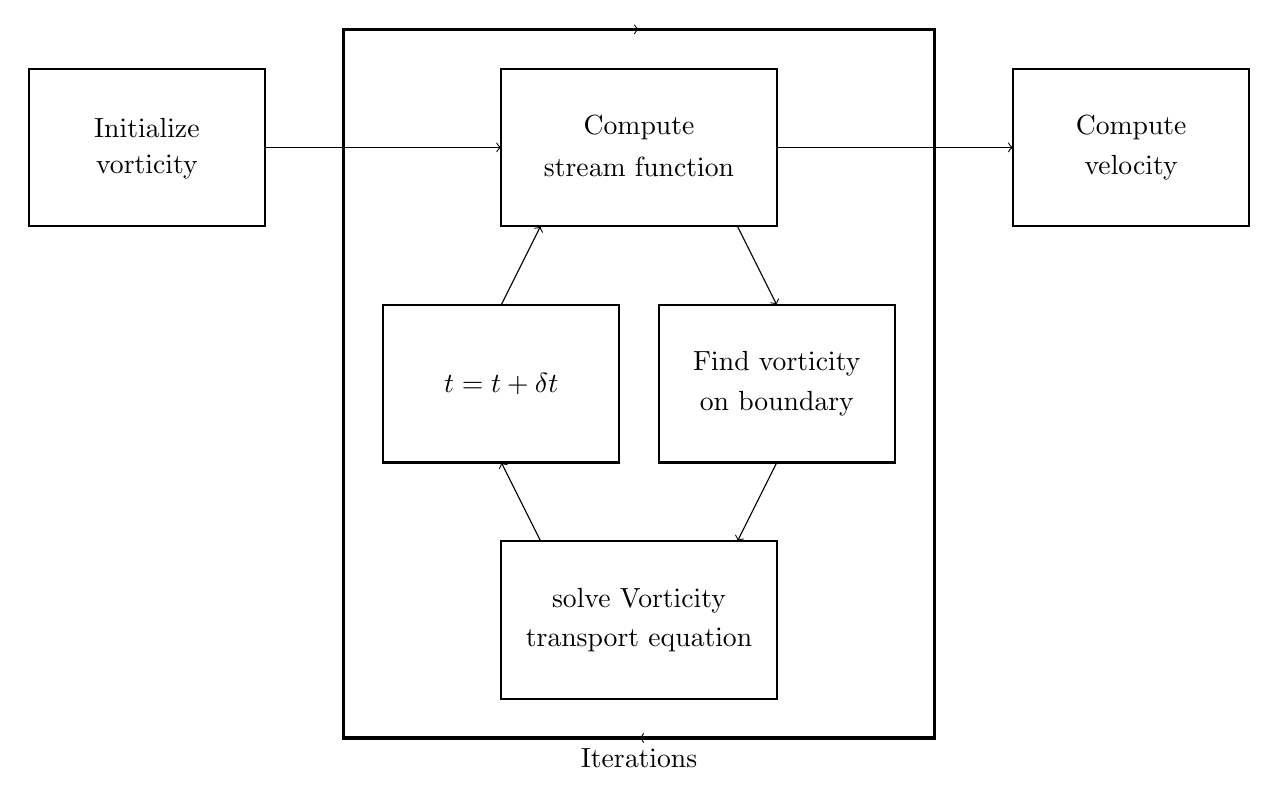
\begin{tikzpicture}
%\draw[step=0.5cm,gray,very thin] (0,0) grid (17,11); %background grid

\draw[very thick] (4.5,1) -- (12,1) -- (12,10) -- (4.5,10) -- cycle; % middle large
\draw[thick] (0.5,7.5) -- (3.5,7.5) -- (3.5,9.5) -- (0.5,9.5) -- cycle; % left
\draw[thick] (13,7.5) -- (16,7.5) -- (16,9.5) -- (13,9.5) -- cycle; % right
\draw[thick] (6.5,7.5) -- (10,7.5) -- (10,9.5) -- (6.5,9.5) -- cycle; % middle top
\draw[thick] (6.5,1.5) -- (10,1.5) -- (10,3.5) -- (6.5,3.5) -- cycle; % middle low
\draw[thick] (5,4.5) -- (8,4.5) -- (8,6.5) -- (5,6.5) -- cycle; % middle left
\draw[thick] (8.5,4.5) -- (11.5,4.5) -- (11.5,6.5) -- (8.5,6.5) -- cycle; % middle right

\node[] at (2,8.75) {Initialize}; \node[] at (2,8.25) {vorticity};
\node[] at (14.5,8.75) {Compute }; \node[] at (14.5,8.25) {velocity};
\node[] at (8.25,8.75) {Compute }; \node[] at (8.25,8.25) {stream function};
\node[] at (10,5.75) {Find vorticity}; \node[] at (10,5.25) {on boundary};
\node[] at (8.25,2.75) {solve Vorticity }; \node[] at (8.25,2.25) {transport equation};
\node[] at (6.5,5.5) {$t=t+ \delta t$}; 
\node[] at (8.25,0.75) {Iterations }; 

\draw [->] (3.5,8.5) -- (6.5,8.5);
\draw [->] (10,8.5) -- (13,8.5);
\draw [->] (9.5,7.5) -- (10,6.5);
\draw [->] (10,4.5) -- (9.5,3.5);
\draw [->] (7,3.5) -- (6.5,4.5);
\draw [->] (6.5,6.5) -- (7,7.5);

\draw [->] (12,1) -- (8.25,1);

\draw [->] (6,10) -- (8.25,10);

\end{tikzpicture}
\end{center}


%%%%%%%%%%%%%%%%%%%%%%%%%%%%%%%%%%%%%%%%%%
\subsection*{benchmark}


Before we solve the problem above we need to make sure that the code is correct. 
After all, we are solving to PDEs with somewhat complex boundary conditions inside a
convergence loop. We here focus on the steady state Navier-Stokes equation and on the Stokes equation. 

Let us now prescribe $u(y)=y(1-y)$ on the inlet, i.e. a flow with a parabolic profile. 
Since the velocity is independent of the $x$-coordinate this implies that all derivatives with respect to $x$ will vanish. 
We then expect this velocity everywhere in the domain since it is solution of the steady state Navier-Stokes and Stokes equations ({\color{orange} todo}), so that 
$\omega (x,y)
= \frac{\partial v}{\partial x} - \frac{\partial u}{\partial y}
= - 1+2y$ anywhere in the domain. 

Since $u=y(1-y) = \frac{\partial \Psi}{\partial y}$ on the boundary and $\Psi$ independent of $x$ there too, I can compute 
$\Psi(y)=\frac12 y^2 - \frac13 y^3 + c$ where $c$ is a constant.
Since $\Psi$ is known up to a constant (and is constant) at the bottom, we arbitrarily fix $\Psi=0$ at the bottom, which automatically sets $c=0$ (continuity of $\Psi$). 
This means that at the top $\Psi$ is constant and equal to $\frac12-\frac13=\frac16$. At the outlet we have $\partial \Psi/\partial x=0$. This last condition is 
compatible with the values on the top and bottom so no need to think about the corners.

We then have the analytical solution for this problem:
\begin{eqnarray}
u(x,y)&=& y(1-y) \nn\\
v(x,y)&=& 0 \nn\\
\Psi(x,y)&=& \frac12 y^2 - \frac13 y^3  \nn\\
\omega(x,y) &=& - 1+2y
\end{eqnarray}
We can use these expressions to check the results of each Poisson solver: 
when solving for $\Psi$ we use the analytical expression for $\omega$, and when 
solving for $\omega$ we can use the analytical expression for $\Psi$. 
In the end we find that each block of the code is correct. 

At this stage the loop goes as follows:
\begin{verbatim}
omega[:]=0
for iter in range(0,niter):
    solve Delta psi = -omega
    compute u,v from psi 
    solve vorticity eq (psi used in bc) -> omega
\end{verbatim}
We find that this simply diverges from the 2nd iteration onwards and ultimately 'explodes' with field values absurdly high.

One way to fix this problem is to use relaxation:
\begin{verbatim}
omega[:]=0
omegamem[:]=0
psimem[:]=0
for iter in range(0,niter):
    solve Delta psi = -omega
    psi[:]=beta*psi[:]+(1-beta)*psimem[:]
    compute u,v from psi 
    solve vorticity eq (psi used in bc) -> omega
    omega[:]=beta*omega[:]+(1-beta)*omegamem[:]
    psimem[:]=psi[:]
    omegamem[:]=omega[:]
\end{verbatim}
where $\beta$ controls the relaxation. If equal to one, there is none. If $\beta\rightarrow 0$ there is little progress being made in the loop towards convergence.
We find that $\beta=0.5$ still diverges but $\beta=0.33$ yields a successful iteration.

Remark: Another avenue could be to think about the first PDE $\Delta \Psi = -\omega$.
Although it is true that we do not know $\omega$ everywhere in the domain it 
could be still beneficial to start with a field $\omega$ that reflects the boundary conditions, i.e. apply the b.c. for $\omega$. Of course some of these b.c. depend on $\Psi$ inside the domain which we obviously do not know, but we can nevertheless give it a try. On 2nd thought, it is somewhat stupid: i can only compute $\omega$ on the boundary which is precisely where psi b.c. are prescribed so that these values 
of omega are not used in the end.

\begin{center}
\includegraphics[width=8cm]{python_codes/fieldstone_154/results/conv.pdf}
\includegraphics[width=8cm]{python_codes/fieldstone_154/results/errors.pdf}\\
{\captionfont Left: convergence of $u$, $v$, $\psi$ and $\omega$ during the iterations. Right: 2-norm of the error fields (i.e. 
computed fields - analytical solution)}
\end{center}

\begin{center}
\includegraphics[width=8cm]{python_codes/fieldstone_154/results/u}
\includegraphics[width=8cm]{python_codes/fieldstone_154/results/v}\\
\includegraphics[width=8cm]{python_codes/fieldstone_154/results/psi}
\includegraphics[width=8cm]{python_codes/fieldstone_154/results/omega}
\end{center}


\begin{center}
\includegraphics[width=8cm]{python_codes/fieldstone_154/results/stats_u}
\includegraphics[width=8cm]{python_codes/fieldstone_154/results/stats_v}\\
\includegraphics[width=8cm]{python_codes/fieldstone_154/results/stats_psi}
\includegraphics[width=8cm]{python_codes/fieldstone_154/results/stats_omega}
\end{center}



%%%%%%%%%%%%%%%%%%%%%%%%%%%%%%%%%%%%%%%%%%%%%%%%
\section*{Donea \& Huerta manufactured solution}

We start from the biharmonic equation 
\[
\vec\nabla^4 \Psi = \frac{1}{\eta_0} \left( -\frac{\partial b_x}{\partial y}
+\frac{\partial b_y}{\partial x} \right)
\]

In Section~\ref{ss:mms_bocg12} we find the stream function 
defined in the unit square
\[
\Psi (x,y)=f(x) \cdot g(y)=x^2(x-1)^2 \cdot y^2(y-1)^2, 
\]
with 
\begin{eqnarray}
f'(x)
&=&2x(x-1)^2+2x^2(x-1) \nn\\
&=&2(x-1)[x(x-1)+x^2]  \nn\\
&=&2(x-1)(2x^2 -x)  \nn\\
&=&2x(x-1)(2x -1)  \nn\\
f''(x)
&=& 2 [ (x-1)(2x -1) + x(2x-1)+2x(x-1)] \nn\\
&=& 2 (2x^2 -x-2x+1 + 2x^2-x+2x^2-2x) \nn\\
&=& 2 (6x^2 -6x +1) \nn\\
f'''(x) &=& 12(2x-1) \nn\\
f''''(x) &=& 24 \nn\\
g'(y)
&=& 2y (y-1)^2 + 2y^2(y-1)  \nn\\
&=& 2(y-1)[y(y-1)+y^2] \nn\\
&=& 2(y-1)(2y^2-y) \nn\\
&=& 2y(y-1)(2y-1) \nn\\
g''(y) 
&=& 2[ (y-1)(2y-1) +y(2y-1)+2y(y-1) ] \nn\\
&=& 2[ 2y^2 - 3y +1 +2y^2-y +2y^2-2y] \nn\\
&=& 2(6y^2 -6y+1) \nn\\
g'''(y) &=& 2(12y-1) \nn\\
g''''(y) &=& 24 \nn
\end{eqnarray}

In what follows we wish to verify that once we have postulated 
a pressure field this stream function is compatible with the 
$\vec{b}$ vector of the Donea \& Huerta benchmark of Section~\ref{mms1}.

We then must compute:
\begin{eqnarray}
\vec\nabla^2 \Psi 
&=& \frac{\partial^2 \Psi}{\partial x^2} +\frac{\partial^2 \Psi}{\partial y^2} \nn\\
&=& \frac{\partial^2 }{\partial x^2} (fg)  +\frac{\partial^2 }{\partial y^2} (fg)\nn\\
&=& f''g+ fg'' \nn\\
\vec\nabla^4 \Psi 
&=& \vec\nabla^2 (f''g+fg'') \nn\\
&=& f''''g +2f''g'' + fg'''' \nn\\
&=&24 y^2(y-1)^2 + 2 \cdot  2 (6x^2 -6x +1)  \cdot 2(6y^2 -6y+1)  + 24 x^2(x-1)^2\nn\\
&=&24 (y^4-2y^3+y^2)+8 (6x^2 -6x +1)  (6y^2 -6y+1)  + 24(x^4 -2x^3 +x^2)\nn\\
&=&24 (y^4-2y^3+y^2)+(288x^2y^2 -288 x^2y +48x^2 -288xy^2 +288xy-48x + 48y^2 -48y+8)+24(x^4 -2x^3+x^2)\nn\\
&=& 8 -48x -48y 
+ 288xy + (48+24)x^2 +(24+48)y^2 
-288x^2y -288xy^2 -48x^3 -48y^3 
+ 288x^2y^2+24x^4 + 24y^4\nn\\
&=& 8 -48x -48y + 288xy + 72x^2 +72y^2  -288x^2y -288xy^2 -48x^3 -48y^3 
+ 288x^2y^2+24x^4 + 24y^4 \nn
\end{eqnarray}
Assuming $\eta_0=1$ the stream function above yields the Donea \& Huerta velocity field:
\begin{eqnarray}
u(x,y) &=& \partial_y \Psi = f(x)g'(y) = x^2(x-1)^2 2y(y-1)(2y-1) \nn\\
v(x,y) &=& -\partial_x \Psi = -f'(x)g(y) = -2x(x-1)(2x -1)y^2(y-1)^2 
\end{eqnarray}
As we have seen when deriving the biharmonic equation the pressure 
entirely disappears by cancellation so we can postulate the pressure field to be 
\[
p(x,y) = \frac12 x^2 -\frac16
\]
Note that the $1/6$ offset is such that $\int p dV = 0$.

The right hand side $\vec{b}$ is to be found in Section~\ref{mms1}:
\begin{eqnarray}
b_x &=& (12 - 24y) x^4 + (-24 + 48y) x^3 + (-48y + 72y^2 - 48 y^3 + 12) x^2 \nonumber\\
    && + (-2 + 24y -72y^2+48y^3)x + 1-4y + 12y^2-8y^3 \nonumber\\ 
b_y &=& (8 - 48y + 48 y^2) x^3 + (-12 + 72y - 72y^2) x^2  \nonumber\\
    && + (4 - 24y + 48y^2 - 48y^3 + 24y^4) x - 12y^2 + 24y^3 - 12y^4  \nonumber
\end{eqnarray}
so that we can compute 
\begin{eqnarray}
\frac{\partial b_x}{\partial y}
&=& -24 x^4 + 48 x^3 + (-48 + 144y - 144 y^2 ) x^2  + ( 24 -144 y+ 144y^2)x -4 + 24y-24y^2 \nn\\ 
&=& -24 x^4 + 48 x^3 -48x^2 + 144x^2y - 144 x^2y^2 +  24x -144x y+ 144xy^2  -4 + 24y-24y^2 \nn\\ 
\frac{\partial b_y}{\partial x} 
&=& (8 - 48y + 48 y^2) 3x^2 + (-12 + 72y - 72y^2) 2x  + (4 - 24y + 48y^2 - 48y^3 + 24y^4)   \nn\\
&=& 24x^2 - 144x^2y + 144x^2 y^2 -24x + 144xy - 144xy^2 + 4 - 24y + 48y^2 - 48y^3 + 24y^4   \nn
\end{eqnarray}
and then 
\begin{eqnarray}
&&{\cal F}(x,y)\nn\\
&=&-\frac{\partial b_x}{\partial y}
+\frac{\partial b_y}{\partial x} \nn\\
&=&(4+4)+(-24-24)x+(-24-24)y+ \nn\\
&&(48+24)x^2 + (24+48)y^2 +(144+144)xy \nn\\
&&+ (-144-144)x^2y + (-144-144)xy^2 + (-48)x^3 + (-48)y^3 \nn\\
&& (144+144)x^2y^2  +(24)x^4+(24)y^4 \nn\\
&=& 8 -48x-48y + 72x^2 +72y^2 + 288 xy -288x^2y -288 xy^2 -48x^3-48y^3 + 288x^2y^2 +24x^4 +24 y^4 \nn
\end{eqnarray}

In the end we wish to solve $\vec\nabla^2 \omega = -{\cal F}(x,y)$ since $\eta_0=1$.












%%%%%%%%%%%%%%%%%%%%%%%%%%%%%%%%%%%%%%%%%%%%%%%%%%%%%%%%%%%%%%%%%%%%%%%%%%%%%%%%%%%%%%%%%%%%%%%%%%%
\par\noindent\rule{\textwidth}{0.4pt}

\vspace{.5cm}

\begin{center}
\fbox{\begin{minipage}{0.9\textwidth}
{\color{teal}To Do, open questions, future work?}
\begin{itemize}
\item N-S case i.e. time dependent ?
\item do original bench
\end{itemize}
\end{minipage}}
\end{center}

